\documentclass{beamer}

\usepackage[english]{babel}
\usepackage[utf8]{inputenc}
\usepackage[T1]{fontenc}
\usepackage{tikz}
\usepackage[overlay,absolute]{textpos}

\usetheme{nescala}
\setbeamercovered{transparent}

\newcommand\fullpicture[1]{
  {
    \setbeamertemplate{background}{}
    \begin{frame}[plain]
      \begin{tikzpicture}[remember picture,overlay]
        \node[at=(current page.center)] {
          \includegraphics[keepaspectratio,height=1.2\paperheight,width=1.2\paperwidth]{#1}
        };
      \end{tikzpicture}
    \end{frame}
  }
}

\begin{document}

  \title{Macros vs Types}
  \author{Eugene Burmako \& Lars Hupel}
  \institute{\'Ecole Polytechnique F\'ed\'erale de Lausanne\\Technische Universit\"at M\"unchen}
  \date{March 1, 2014}

{
\setbeamertemplate{footline}{}
\begin{frame}
  \titlepage

  \begin{center}
    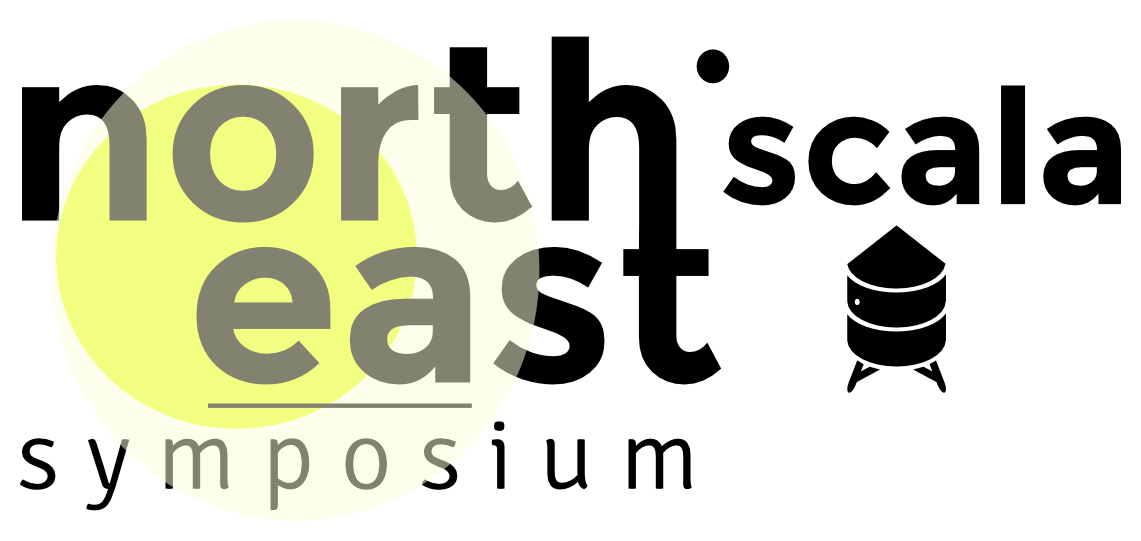
\includegraphics[width=2cm]{img/nescala-logo.png}
  \end{center}
\end{frame}
}

\begin{frame}{Macros vs types}
  \begin{itemize}
    \item Types have been used to metaprogram Scala for ages
    \item Macros are the new player on the field
    \item Debates are hot in the IRC and on Twitter
    \item Time to figure out who's the best once and for all!
  \end{itemize}
\end{frame}

\begin{frame}{Let the games begin!}
  Following the \text{\color{blue}\href{http://scalamacros.org/paperstalks/2014-02-04-WhatAreMacrosGoodFor.pdf}{``What are macros good for?''}} talk, we will see how the contenders fare in three disciplines:

  \vspace{1em}
  \begin{itemize}
    \item Code generation
    \item Static checks
    \item Domain-specific languages
  \end{itemize}
\end{frame}

\AtBeginSection[]
{
  \begin{frame}
    \vskip40pt
    \begin{center}
      \usebeamercolor[fg]{structure}{\Large{\insertsection}}
    \end{center}
  \end{frame}
}

  \section{Code generation}


\begin{frame}[fragile]{Code generation}
  Every language ecosystem has it\visible<2>{, even Haskell
    \vspace{1em}
    \begin{itemize}
      \item \texttt{lens}

         derive lenses for fields of a data type
      \item \texttt{yesod}

        templating, routing
      \item \texttt{invertible-syntax}

        constructing partial isomorphisms for constructors
    \end{itemize}
  }
\end{frame}

\begin{frame}[fragile]{Textual code generation}{Example: Parser generators}
  % from Tom Niemann <epaperpress.com>
  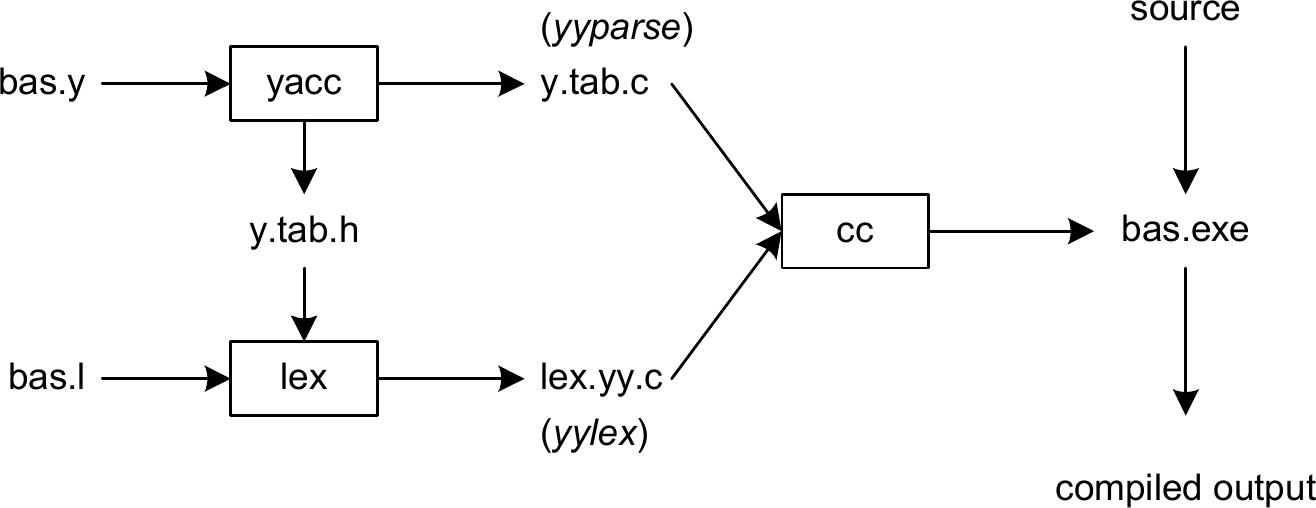
\includegraphics[width=\linewidth]{img/yacc.png}
\end{frame}

\begin{frame}[fragile]{Textual codegen is too low-tech}
  \begin{itemize}
    \item Easy to mess up when concatenating strings
    \item Little knowledge about the program being compiled
    \item Needs to be hooked into the build process
    \item We need a better solution!
  \end{itemize}
\end{frame}

\begin{frame}{Enter types}
  \begin{itemize}
    \item Scala's type system is Turing-complete
    \item This enables some form of code generation
    \item But it's not particularly straightforward
  \end{itemize}
\end{frame}

% TODO Do we want to provide an example here?

\begin{frame}{Enter macros}
  \begin{itemize}
    \item Functions that are run at compile time
    \item Operate on abstract syntax trees not on strings
    \item Communicate with compiler to learn things about the program
    \item A lot of popular Scala libraries are already using macros
  \end{itemize}
\end{frame}

\begin{frame}[fragile]{Use case: Specialization}
  Specialization helps with writing high-performance code,
  but it bloats the code significantly

  \vspace{1em}
  \begin{verbatim}
def mkArray[@specialized T: ClassTag](size: Int, el: T) = {
  val a = new Array[T](size)
  for (i <- 0 until size) a(i) = el
  a
}
  \end{verbatim}
\end{frame}

\begin{frame}[fragile]{Use case: Specialization}
  With macros we can write a specialization code generator ourselves,
  having fine-grained control over what we're specializing

  \vspace{1em}
  \begin{semiverbatim}
def specialized[T: ClassTag](code: => T) = macro ...

def mkArray[T: ClassTag](size: Int, el: T) = \{
  val a = new Array[T](size)
  \text{\color{blue}{specialized[T] \{}}
    for (i <- 0 until size) a(i) = el
  \text{\color{blue}{\}}}
  a
\}
  \end{semiverbatim}
\end{frame}

\begin{frame}{What are types bringing into the mix?}
  \begin{itemize}
    \item Thanks to macros code generation becomes accessible and fun
    \item But: Macros are essentially opaque to humans
    \item We can and should try to alleviate this with types
  \end{itemize}
\end{frame}

\begin{frame}{Use case: Materialization}
  We want to have: default implementations for
  \begin{itemize}
    \item \texttt{Semigroup} (pointwise addition)
    \item \texttt{Ordering} (lexicographic order)
    \item \texttt{Binary} (pickling/unpickling)
  \end{itemize}

  \vspace{1em}
  We do not want to: write boilerplate
  \begin{itemize}
    \item Repetitive \& error-prone
  \end{itemize}
\end{frame}

\begin{frame}{Use case: Materialization}
  \texttt{scalac} already synthesizes \texttt{equals}, \texttt{toString} ...

  \vspace{1em}
  \begin{alertblock}{Problem}<visible@2->
    Not extensible
  \end{alertblock}

  \vspace{1em}
  \begin{exampleblock}{Solution}<visible@3->
    Materialization based on type classes and implicit macros
  \end{exampleblock}
\end{frame}

\begin{frame}{Type classes \`a la Scala}
  \begin{itemize}
    \item Type classes are (first-class) traits
    \item Instances are (first-class) values
    \item<visible@2> \text{\color{blue}{Both can use arbitrary language features}}
  \end{itemize}
\end{frame}

\begin{frame}[fragile]{Use case: Materialization}
  \begin{verbatim}
implicit def derive[C[_] : TypeClass, T]: C[T] =
  macro TypeClass.derive_impl[C, T]
  \end{verbatim}
\end{frame}

\begin{frame}{The power of materialization}
  \begin{itemize}
    \item First introduced in Shapeless
    \item Similar to \texttt{deriving Eq} in Haskell
    \item Extensible without modifying the macro(s) itself
  \end{itemize}
\end{frame}

\begin{frame}[fragile]{The dangers of materialization}
  \vspace{1em}
  \begin{alertblock}{Bad}
    \begin{verbatim}
implicit def derive[C[_], T]: C[T] =
  macro TypeClass.derive_impl[C, T]
    \end{verbatim}
  \end{alertblock}

  \vspace{1em}
  \begin{exampleblock}{Good}
    \begin{semiverbatim}
implicit def derive[C[_] : \text{\color{blue}{TypeClass}}, T]: C[T] =
  macro TypeClass.derive_impl[C, T]
    \end{semiverbatim}
  \end{exampleblock}
\end{frame}

\begin{frame}[fragile]{Our advice}
  \begin{itemize}
    \item Macros are great, but are essentially opaque to humans
    \item Try to document the codegen surface using types\\
      (type classes and other advanced techniques really help here!)
    \item Try to limit the codegen surface encapsulating ``moving parts''\\
      (maybe more boilerplate, but more predictable)
    \item Needs best practices for documentation \& testing
  \end{itemize}
\end{frame}

%\begin{frame}{Open problems}
%  % TODO how do we present that?
%  \begin{itemize}
%    \item Best practices for documentation \& testing
%    \item Do we need a compile-time ScalaCheck?
%  \end{itemize}
%\end{frame}

  \section{Static checks}

\begin{frame}{Types \`a la Pierce}
  \begin{quote}
    ``A type system is a tractable syntactic method for \text{\color<2>{blue}{proving the absence of certain program behaviors}} by classifying phrases according to the kinds of values they compute.''
  \end{quote}
  \hfill -- Benjamin Pierce, in: Types and Programming Languages
\end{frame}

\begin{frame}{Types \`a la Scala}
  Scala has a sophisticated type system
  \begin{itemize}
    \item Path-dependent types
    \item Type projections
    \item Higher-kinded types
    \item Implicit parameters
  \end{itemize}
\end{frame}

\begin{frame}{Type computations}
  Implicits allow computations in the type system

  \begin{itemize}
    \item Higher-order unification (\href{https://issues.scala-lang.org/browse/SI-2712}{SI-2712})
    \item Generic operations on tuples
    \item Extensible records
    \item Statically size-checked collections
  \end{itemize}
\end{frame}

\begin{frame}{Shapeless}
  The library that makes advanced types accessible!
\end{frame}

\begin{frame}[fragile]{Type computations}{Example: Sized collections}
  \begin{verbatim}
// typed as Sized[_2, List[String]]
val hdrs = Sized("Title", "Author")

// typed as List[Sized[_2, List[String]]]
val rows = List(
  Sized("TAPL", "B. Pierce"),
  Sized("Implementation of FP Languages", "SPJ")
)
  \end{verbatim}

  % TODO Maybe collection operation on tuples or records? These are my personal favorites in Shapeless.
\end{frame}

\begin{frame}{The power of type computation}
  Computing with implicits is sometimes called ``Poor Man's Prolog''
  \vspace{1em}

  But: Almost anything can be done

  % TODO Not sure whether I follow
\end{frame}

% <https://secure.flickr.com/photos/mszeto/3261725397/>
\fullpicture{img/hanoi.jpg}

\begin{frame}{What are macros bringing into the mix?}
  \begin{itemize}
    \item Type system doesn't cover everything
    \item Complex type computations are hard to debug

      (sometimes, \texttt{-Xlog-implicits} is not enough)
    \item Implicit-heavy code slows down compiler significantly
  \end{itemize}
\end{frame}

\begin{frame}[fragile]
\frametitle<1>{Let's overthrow the tyranny of types!}
\frametitle<2>{Completely replacing types with macros: not a good idea}
  Macros can do anything, including validation of arguments,\\
  so we shouldn't bother with all those complex types anymore

  \vspace{1em}
  \begin{alertblock}{Bad}
    \begin{verbatim}
trait GenTraversableLike[+A, +Repr] {
  def map[B, R](f: A => B)
    (implicit bf: CanBuildFrom[Repr, B, R]): R
}
    \end{verbatim}
  \end{alertblock}

  \begin{exampleblock}{Good}
    \begin{semiverbatim}
trait GenTraversableLike \{
  def map(f: Any): Any = \text{\color{blue}{macro}} ...
\}
    \end{semiverbatim}
  \end{exampleblock}

  \begin{textblock*}{\textwidth}(15mm,10mm)
    \begin{visibleenv}<2->
      % from https://upload.wikimedia.org/wikipedia/commons/7/79/Operation_Upshot-Knothole_-_Badger_001.jpg
      
\includegraphics[height=8cm]{img/boom.jpg}
    \end{visibleenv}
  \end{textblock*}
\end{frame}

\begin{frame}[fragile]{Reasonable use case: Checked arithmetics}
  Spire provides a \texttt{checked} macro to detect arithmetic overflows.
  Types can't capture this, so it's okay to use a macro here.

  \vspace{1em}
  \begin{verbatim}
// returns None when x + y overflows
Checked.option {
  x + y < z
}
  \end{verbatim}
\end{frame}

% TODO
%\begin{frame}{Reasonable use case: Example of short-circuiting computations with macros}
%  What would be the best example from shapeless here?
%\end{frame}

\begin{frame}{Our advice}
  \begin{itemize}
  \item For static checks use types whenever possible
  \item Macros if impossible or heavyweight
  \item Try to document and encapsulate the magic using types\\
        (type classes are particularly nice for this purpose)
  \end{itemize}
\end{frame}

  \section{Domain-specific languages}

\begin{frame}{Domain-specific languages}
  As per ``DSLs in Action'':
  \begin{itemize}
  \item \text{\color<2>{blue}{Embedded aka internal}}\only<2>{\text{\color{blue}{ <- in this talk}}}
  \item Standalone aka external
  \item Non-textual
  \end{itemize}
\end{frame}

\begin{frame}[fragile]{Use case: Slick}{An embedded DSL for data access}
  \vspace{1em}
  \begin{alertblock}{Instead of writing database code in SQL}
    \begin{verbatim}
select c.NAME from COFFEES c where c.ID = 10
    \end{verbatim}
  \end{alertblock}

  \vspace{1em}
  \begin{exampleblock}{Write database code in Scala}
    \begin{verbatim}
for (c <- coffees if c.id == 10) yield c.name
    \end{verbatim}
  \end{exampleblock}
\end{frame}

\begin{frame}{Three approaches}
  \begin{itemize}
  \item Lifted embedding (types)
  \item Direct embedding (macros)
  \item Shadow embedding (macros + types)
  \end{itemize}
\end{frame}

\begin{frame}[fragile]{Lifted embedding (types)}{Types can do domain-specific validation and virtualization}
  \vspace{1em}
  \begin{exampleblock}{Domain rules are encoded in an extra layer of types}
  \begin{semiverbatim}
object Coffees extends Table[\text{\color{blue}{(Int, String, ...)}}] \{
  def id = \text{\color{blue}{column}}[Int]("ID", O.PrimaryKey)
  def name = \text{\color{blue}{column}}[String]("NAME")
  ...
\}
  \end{semiverbatim}
  \end{exampleblock}
\end{frame}

\begin{frame}[fragile]{Lifted embedding (types)}{Types are quite heavyweight under the covers}
  \vspace{1em}
  \begin{exampleblock}{What you write in a Slick DSL}
    \begin{verbatim}
Query(Coffees) filter
  (c => c.id === 10) map
  (c => c.name)
)\end{verbatim}
  \end{exampleblock}

  \vspace{1em}
  \begin{alertblock}{What actually happens under the covers}
    \begin{semiverbatim}
Query(Coffees) filter
  (c => c.id: \text{\color{blue}{Column[Int]}} === 10: \text{\color{blue}{Column[Int]}}) map
  (c => c.name: \text{\color{blue}{Column[String]}})
    \end{semiverbatim}
  \end{alertblock}
\end{frame}

\begin{frame}[fragile]{Lifted embedding (types)}{Types can be really bad at error messages}
  \vspace{1em}
  \begin{exampleblock}{Trying to compile}
    \begin{verbatim}
Query(Coffees) map (c =>
  if (c.origin === "Iran") "Good"
  else c.quality
)\end{verbatim}
  \end{exampleblock}

  \vspace{1em}
  \begin{alertblock}{Produces the following error}
    \begin{verbatim}
Don't know how to unpack Any to T and pack to G
not enough arguments for method map: (implicit shape:
slick.lifted.Shape[Any,T,G]) slick.lifted.Query[G,T].
Unspecified value parameter
    \end{verbatim}
  \end{alertblock}

  % This happens because vanilla ifs aren't supported by lifted embedding,
  % but that doesn't follow from the error message
\end{frame}

\begin{frame}[fragile]{Direct embedding (macros)}{Macros can also validate and virtualize Scala code}
  \vspace{1em}
  \begin{exampleblock}{Type signatures are simple and error messages are to the point}
  \begin{semiverbatim}
case class Coffee(id: Int, name: String, ...)

Query[Coffee] filter
  (c => c.id: \text{\color{blue}{Int}} == 10: \text{\color{blue}{Int}}) map
  (c => c.name: \text{\color{blue}{String}})
  \end{semiverbatim}
  \end{exampleblock}
\end{frame}

\begin{frame}[fragile]{Direct embedding (macros)}{Macros can do static checks, but sometimes that's non-trivial to get right}
  \vspace{1em}
  \begin{exampleblock}{Trying to use an unsupported feature}
  \begin{semiverbatim}
Query[Coffee] map
  (c => c.id\text{\color{blue}{.toDouble}})
  \end{semiverbatim}
  \end{exampleblock}

  \vspace{1em}
  \begin{alertblock}{Crashes at runtime}
  \vspace{1em}
  This is what we get when we try to reinvent types
  \end{alertblock}

  \begin{textblock*}{\textwidth}(15mm,10mm)
    \begin{visibleenv}<2->
      % from https://upload.wikimedia.org/wikipedia/commons/7/79/Operation_Upshot-Knothole_-_Badger_001.jpg
      
\includegraphics[height=8cm]{img/boom.jpg}
    \end{visibleenv}
  \end{textblock*}
\end{frame}

\begin{frame}[fragile]{Shadow embedding (macros + types)}{Based on YinYang, which uses macros and therefore enjoys all benefits of macros}
  \vspace{1em}
  \begin{exampleblock}{Type signatures are simple and error messages are to the point}
  \begin{semiverbatim}
case class Coffee(id: Int, name: String, ...)

slick \{
  Query[Coffee] filter
    (c => c.id: \text{\color{blue}{Int}} == 10: \text{\color{blue}{Int}}) map
    (c => c.name: \text{\color{blue}{String}})
  \}
\}\end{semiverbatim}
  \end{exampleblock}
\end{frame}

\begin{frame}[fragile]{Shadow embedding (macros + types)}{Uses types to moderate APIs available inside DSL blocks}
  \vspace{1em}
  \begin{exampleblock}{DSL author specifies the set of available APIs using types}
  \begin{semiverbatim}
// In Scala's standard library (front-end)
final abstract class Int private extends AnyVal \{
  ...
  def toDouble: Double
  ...
\}

// In Slick's lifted embedding (back-end)
Value toDouble is not a member of Column[Int].
  \end{semiverbatim}
  \end{exampleblock}
\end{frame}

\begin{frame}[fragile]{Shadow embedding (macros + types)}{The best of two worlds}
  \vspace{1em}
  \begin{exampleblock}{Trying to do something unsupported}
  \begin{semiverbatim}
slick \{
  Query[Coffee] map
    (c => c.id\text{\color{blue}{.toDouble}})
\}\end{semiverbatim}
  \end{exampleblock}

  \vspace{1em}
  \begin{exampleblock}{Produces comprehensible and comprehensive errors}
  \begin{semiverbatim}
in Slick method toDouble is not a member of Int
  \end{semiverbatim}
  \end{exampleblock}
\end{frame}

\begin{frame}[fragile]{Shadow embedding (macros + types)}{An important limitation of the current macro system}
  \vspace{1em}
  \begin{alertblock}{Macros can't see ASTs of everything in the program}
  \begin{semiverbatim}
def idIsTen(c: Coffee) = c.id == 10

slick \{
  Query[Coffee] filter \text{\color{blue}{idIsTen}}
\}
  \end{semiverbatim}
  \end{alertblock}
\end{frame}

\begin{frame}{Our advice}
  \begin{itemize}
  \item Types work, but sometimes become too heavyweight\\
        both for the DSL author and for the users
  \item With macros a lot of traditional ceremony is unnecessary,\\
        and that makes DSL development faster and more productive
  \item But: Macros currently have inherent problems with modularity\\
        (we're working on this, see my tomorrow's talk!)
  \item If you decide to go with macros, always try to document and encapsulate
        macro magic with types as much as possible
  \end{itemize}
\end{frame}

  \section{Summary}

\begin{frame}[fragile]{Types are more declarative, but less powerful}
  \begin{center}
    % from http://da.wallpapersus.com/magnetic-field/
    
\includegraphics[height=6cm]{img/magnet.jpg}
  \end{center}
\end{frame}

\begin{frame}[fragile]{Macros are more powerful, but less declarative}
  \begin{center}
    % from https://upload.wikimedia.org/wikipedia/commons/7/79/Operation_Upshot-Knothole_-_Badger_001.jpg
    
\includegraphics[height=8cm]{img/boom.jpg}
  \end{center}
\end{frame}

\begin{frame}[fragile]{Use whatever's simpler, try combining strong points of both}
  \begin{center}
    % from http://newsicare.wordpress.com/2010/07/14/building-the-open-source-bussard-fusion-reactor/
    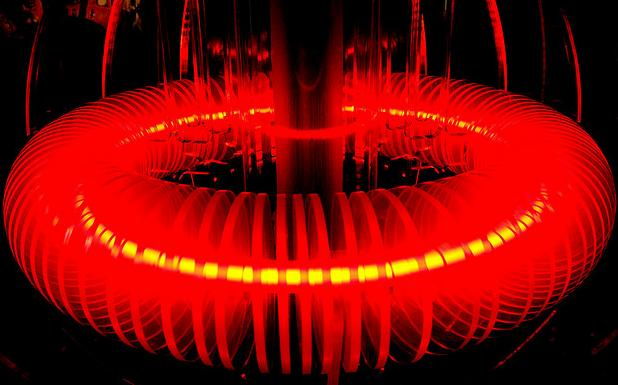
\includegraphics[height=6.5cm]{img/fusion.jpg}
  \end{center}
\end{frame}

\begin{frame}{Credits}

\begin{itemize}
\item Thanks to \text{\color{blue}\href{https://github.com/amirsh/master-thesis}{Amir Shaikhha}} for the shadow embedding thesis
\item Thanks to \text{\color{blue}\href{https://github.com/vjovanov/yin-yang}{Vojin Jovanovic}} and \text{\color{blue}\href{https://github.com/szeiger}{Stefan Zeiger}} for DSL help
\item Thanks to \text{\color{blue}\href{https://github.com/densh}{Denys Shabalin}} and others for their comments
\item Thanks to \text{\color{blue}\href{http://epaperpress.com/}{Tom Niemann}} for the parser generators diagram
\item Thanks to \text{\color{blue}\href{https://secure.flickr.com/photos/mszeto/3261725397}{Flickr}} for the Hanoi towers picture
\item Thanks to \text{\color{blue}\href{http://da.wallpapersus.com/magnetic-field/}{wallpapersus.com}} for the magnet picture
\item Thanks to \text{\color{blue}\href{https://upload.wikimedia.org/wikipedia/commons/7/79/Operation_Upshot-Knothole_-_Badger_001.jpg}{Wikipedia}} for the nuclear explosion picture
\item Thanks to \text{\color{blue}\href{http://newsicare.wordpress.com/2010/07/14/building-the-open-source-bussard-fusion-reactor}{Flickr}} for the fusion reactor picture
\item Thanks to you for reading and listening :)
\end{itemize}
\end{frame}

% TODO: we need to have a slide with credits:
% * sources of images
% * credits to Amir for his examples in the DSL section
% * thanks to Denys, Vojin and Stefan for reviews

\end{document}
